\subsection{Baire Category}

\begin{definition} \label{def:fsigma-gdelta-nowhere-dense} \hlt{$F_\sigma$, $G_\delta$, and Nowhere-Dense Sets}\\
For subsets of a metric space $X$:
\begin{enumerate}[label=(\roman*)]
\setlength{\itemsep}{0pt}
\item $A$ is an \hlt{$F_\sigma$ set} if $A=\bigcup_{n=1}^{\infty}F_n$ for closed sets $F_n$.
\item $B$ is a \hlt{$G_\delta$ set} if $B=\bigcap_{n=1}^{\infty}G_n$ for open sets $G_n$.
\item $E$ is \hlt{nowhere dense} if $(\overline{E})^\circ=\emptyset$; equivalently, no nonempty open set is contained in $\overline{E}$.
\end{enumerate}
For $X=\R$, this says exactly that $\overline{E}$ contains no nonempty open interval.
\end{definition}

\begin{proposition} \label{prop:open-real-sets-are-fsigma} \hlt{Open Real Sets Are $F_\sigma$}\\
For subsets of $\R$:
\begin{enumerate}[label=(\roman*)]
\setlength{\itemsep}{0pt}
\item If $G\subseteq\R$ is open, then $G$ is $F_\sigma$.
\item If $A\subseteq\R$ is closed, then $A$ is $G_\delta$.
\end{enumerate}
\begin{proof}
\begin{enumerate}[label=(\roman*)]
\setlength{\itemsep}{0pt}
\item If $G=\R$, then $G=\bigcup_{m\geq1}[-m,m]$.\\
Otherwise set $C\defeq\R\setminus G$ and $F_m\defeq[-m,m]\cap\{x\in\R:\operatorname{dist}(x,C)\geq 1/m\}$ for $m\geq1$.\\
The map $x\mapsto\operatorname{dist}(x,C)$ is continuous since $\abs{\operatorname{dist}(x,C)-\operatorname{dist}(y,C)}\leq\abs{x-y}$; hence each $F_m$ is closed.\\
Moreover $F_m\subseteq G$. For $x\in G$, $r>0$ with $(x-r,x+r)\subseteq G$, $m\geq\abs{x}$; $1/m\leq r$ give $x\in F_m$. QED.
\item If $A$ is closed, then $A^c=\bigcup_{m=1}^{\infty}F_m$ with $F_m$ closed by (i), hence $A=\bigcap_{m=1}^{\infty}F_m^c$ is $G_\delta$.
\end{enumerate}
\hlt{Structural Commentary}: Positive distance from the complement gives closed exhaustion.\\
\hlt{Key Insight}: Distance to the complement converts local openness into a countable closed exhaustion.
\end{proof}
\end{proposition}

\begin{definition} \label{def:first-category-set} \hlt{First Category}\\
Let $X$ be a metric space and let $E\subseteq X$. The set $E$ is \hlt{of first category}, \hlt{meager}, or \hlt{thin} in $X$ if there are nowhere-dense sets $N_n\subseteq X$ such that $E\subseteq\bigcup_{n=1}^{\infty}N_n$.\\
\hlt{Structural Commentary}: Meagerness is relative to the ambient space $X$.\\
\hlt{Key Insight}: The Baire Category Theorem says a nonempty complete metric space is not meager in itself.
\end{definition}

\begin{definition} \label{def:residual-thick-generic-set} \hlt{Residual, Thick, and Generic Sets}\\
Let $X$ be a metric space.
\begin{enumerate}[label=(\roman*)]
\setlength{\itemsep}{0pt}
\item A set $G\subseteq X$ is \hlt{residual}, or \hlt{thick}, in $X$ if there are dense open sets $O_n\subseteq X$ such that $\bigcap_{n=1}^{\infty}O_n\subseteq G$.
\item A property $P$ is \hlt{generic} in $X$ if $\{x\in X:P(x)\}$ is residual in $X$.
\end{enumerate}
If $X$ is complete, then every residual subset of $X$ is dense by Theorem \ref{thm:dense-open-baire-complete-metric-space}.\\
\hlt{Key Insight}: Meager sets are topologically small; residual sets contain a countable dense-open core.
\end{definition}

\begin{theorem} \label{thm:dense-open-baire-real-line}\label{thm:completeness-and-baire-source-todo} \hlt{Dense Open Intersections in $\R$}\\
If $G_1,G_2,G_3,\ldots$ are dense open subsets of $\R$, then $\bigcap_{n=1}^{\infty}G_n\neq\emptyset$.
\begin{proof}
We construct nested closed intervals. Since $G_1$ is dense and open, $G_1\cap(0,1)$ contains a nonempty open interval; choose a closed interval $I_1\subseteq G_1\cap(0,1)$ with nonempty interior.\\
Given $I_n=[a_n,b_n]$, density of $G_{n+1}$ gives a point of $G_{n+1}$ in $(a_n,b_n)$. Since $G_{n+1}$ is open, choose a closed interval $I_{n+1}\subseteq G_{n+1}\cap(a_n,b_n)$ with nonempty interior and length $<1/(n+1)$.\\
Then $I_1\supseteq I_2\supseteq I_3\supseteq\cdots$, so Theorem \ref{thm:nested-closed-intervals-intersect} gives $x\in\bigcap_n I_n$. Since $I_n\subseteq G_n$ for every $n$, this $x$ lies in $\bigcap_nG_n$.\\
\hlt{Structural Commentary}: Dense openness builds nested intervals; completeness keeps a limit point.\\
\hlt{Key Insight}: A countable dense-open intersection cannot be destroyed one interval at a time.
\end{proof}
\end{theorem}

\begin{theorem} \label{thm:dense-open-baire-complete-metric-space} \hlt{Dense Open Intersections in Complete Metric Spaces}\\
Let $(X,d)$ be complete, let $O_1,O_2,\ldots$ be dense open subsets of $X$, and let $U\subseteq X$ be nonempty and open.\\
Then $U\cap\bigcap\limits_{n=1}^{\infty}O_n\neq\emptyset$. Consequently, $\bigcap\limits_{n=1}^{\infty}O_n$ is dense in $X$.
\begin{proof}
Choose $x_1\in U\cap O_1$ and $0<r_1<1$ with $C_1\defeq\overline{B}_{r_1}(x_1)\subseteq U\cap O_1$.\\
Inductively, if $C_n=\overline{B}_{r_n}(x_n)\subseteq U\cap O_1\cap\cdots\cap O_n$ and $0<r_n<2^{-n}$, density and openness of $O_{n+1}$ give $x_{n+1}\in B_{r_n}(x_n)\cap O_{n+1}$ and $0<r_{n+1}<2^{-(n+1)}$ such that $C_{n+1}\defeq\overline{B}_{r_{n+1}}(x_{n+1})\subseteq B_{r_n}(x_n)\cap O_{n+1}$.\\
Then $C_{n+1}\subseteq C_n$. If $m>n$, then $x_m\in B_{r_n}(x_n)$, so $d(x_m,x_n)<2^{-n}$; hence $(x_n)$ is Cauchy. Let $x_n\to x$.\\
Since each $C_n$ is closed and contains all sufficiently late $x_m$, we have $x\in C_n$ for every $n$. Thus $x\in U\cap\bigcap_nO_n$.\\
Since every nonempty open $U$ meets $\bigcap_nO_n$, the intersection is dense.\\
\hlt{Structural Commentary}: The interval proof becomes a nested closed-ball proof.\\
\hlt{Key Insight}: Dense open sets choose the next ball; completeness supplies the limiting point.
\end{proof}
\end{theorem}

\begin{figure}[H]
  \centering
  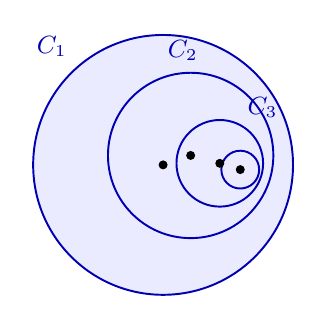
\begin{tikzpicture}[
  every node/.style={font=\small},
  ball/.style={draw=blue!70!black, fill=blue!8, line width=0.7pt},
  center/.style={circle, fill=black, inner sep=1.15pt}
]
  \draw[ball] (0,0) circle (1.65);
  \draw[ball] (0.35,0.12) circle (1.05);
  \draw[ball] (0.72,0.02) circle (0.55);
  \draw[ball] (0.98,-0.06) circle (0.24);

  \node[center] at (0,0) {};
  \node[center] at (0.35,0.12) {};
  \node[center] at (0.72,0.02) {};
  \node[center] at (0.98,-0.06) {};

  \node[blue!70!black, above left] at (-1.1,1.25) {$C_1$};
  \node[blue!70!black, above] at (0.25,1.20) {$C_2$};
  \node[blue!70!black, above right] at (0.95,0.48) {$C_3$};
\end{tikzpicture}

  \caption{Nested closed balls shrink to \(p\).}
  \label{fig:baire-nested-closed-balls}
\end{figure}

\begin{theorem} \label{thm:baire-category-complete-metric-space} \hlt{Baire Category Theorem for Complete Metric Spaces}\\
A nonempty complete metric space is not the union of a countable collection of nowhere-dense sets.
\begin{proof}
Suppose $X=\bigcup_nE_n$ with each $E_n$ nowhere dense, and set $O_n\defeq(\overline{E_n})^c$.\\
Then each $O_n$ is dense open: it is open, and every nonempty open set meets it because no such set lies in $\overline{E_n}$.\\
By Theorem \ref{thm:dense-open-baire-complete-metric-space}, choose $x\in\bigcap_nO_n$. Then $x\notin E_n$ for all $n$, contradicting $X=\bigcup_nE_n$.\\
\hlt{Structural Commentary}: Countably many nowhere-dense sets have dense open complements.\\
\hlt{Key Insight}: Completeness forbids countable assembly from thin pieces.
\end{proof}
\end{theorem}

\begin{corollary} \label{cor:baire-closed-cover-has-interior} \hlt{Closed Cover Interior Test}\\
Let $X$ be a complete metric space and let $(F_n)_{n\in\N}$ be closed subsets of $X$.
\begin{enumerate}[label=(\roman*)]
\setlength{\itemsep}{0pt}
\item If $\emptyset\neq U\subseteq X$ is open and $U\subseteq\bigcup_{n=1}^{\infty}F_n$, then $F_N^\circ\neq\emptyset$ for some $N\in\N$.
\item If $X\neq\emptyset$ and $F_n^\circ=\emptyset$ for every $n\in\N$, then $X\neq\bigcup_{n=1}^{\infty}F_n$.
\end{enumerate}
\begin{proof}
\begin{enumerate}[label=(\roman*)]
\setlength{\itemsep}{0pt}
\item[$(i)$] Assume $\emptyset\neq U\subseteq X$ is open and $U\subseteq\bigcup_{n=1}^{\infty}F_n$. Suppose $F_n^\circ=\emptyset$ for every $n$ and set $O_n\defeq X\setminus F_n$. Since $F_n$ is closed, $O_n$ is open. If $V\subseteq X$ nonempty and open, then $V\nsubseteq F_n$, so $V\cap O_n\neq\emptyset$; hence $O_n$ dense.\\
Theorem \ref{thm:dense-open-baire-complete-metric-space} gives $x\in U\cap\bigcap_{n=1}^{\infty}O_n$. Then $x\in U\subseteq\bigcup_{n=1}^{\infty}F_n$ and $x\notin F_n$ $\forall n$, contradiction. QED.
\item[$(ii)$] Assume $X\neq\emptyset$ and $F_n^\circ=\emptyset$ for every $n$. If $X=\bigcup_{n=1}^{\infty}F_n$, then (i) with $U=X$ gives $F_N^\circ\neq\emptyset$ for some $N$, a contradiction. Hence $X\neq\bigcup_{n=1}^{\infty}F_n$.
\end{enumerate}
\hlt{Structural Commentary}: Empty interiors give dense open complements.\\
\hlt{Key Insight}: Baire forces one complement-avoiding point.
\end{proof}
\end{corollary}

\begin{theorem} \label{thm:baire-local-uniform-boundedness-continuous-family} \hlt{Pointwise Bounded Families Are Locally Uniformly Bounded}\\
Let $(X,d)$ be a nonempty complete metric space, and let $\mathcal{F}\subseteq C(X,\R)$.\\
Assume that for every $x\in X$ there is $M_x<\infty$ such that $\abs{f(x)}\leq M_x$ for every $f\in\mathcal{F}$.\\
Then there exist a nonempty open set $O\subseteq X$ and $M<\infty$ such that $\abs{f(x)}\leq M$ for all $x\in O$ and $f\in\mathcal{F}$.
\begin{proof} For $n\in\N$, set $E_n\defeq\{x\in X:\forall f\in\mathcal{F},\ \abs{f(x)}\leq n\}$.\\
As $E_n=\bigcap_{f\in\mathcal{F}}\{x\in X:\abs{f(x)}\leq n\}$ and each $f$ is continuous, $E_n$ is closed. The hypothesis gives $X=\bigcup_{n=1}^{\infty}E_n$.\\
By Corollary \ref{cor:baire-closed-cover-has-interior}, $E_N^\circ\neq\emptyset$ for some $N\in\N$. Take $O\defeq E_N^\circ$, $M\defeq N$. Then $x\in O$ and $f\in\mathcal{F}$ imply $\abs{f(x)}\leq M$.\\
\hlt{Structural Commentary}: Pointwise bounds form a closed cover.\\
\hlt{Key Insight}: Completeness turns pointwise control into uniform control somewhere.
\end{proof}
\end{theorem}

\begin{theorem} \label{thm:pointwise-limit-continuous-on-dense-set} \hlt{Dense Continuity Set for Pointwise Limits}\\
Let $(X,d)$ be a complete metric space, let $f:X\to\R$, let $f_n:X\to\R$ be continuous for every $n\in\N$, and assume $f_n(x)\to f(x)$ for every $x\in X$. Then there exists $D\subseteq X$ such that:
\begin{enumerate}[label=(\roman*)]
\setlength{\itemsep}{0pt}
\item $D$ is dense in $X$;
\item $(f_n)$ is equicontinuous at every $x_0\in D$;
\item $f$ is continuous at every $x_0\in D$.
\end{enumerate}
\begin{proof} For $m,n\in\N$, set $E_{m,n}\defeq\{x\in X:\forall j,k\geq n,\ \abs{f_j(x)-f_k(x)}\leq 1/m\}$.\\
Since $E_{m,n}=\bigcap_{j,k\geq n}\{x\in X:\abs{f_j(x)-f_k(x)}\leq 1/m\}$, each $E_{m,n}$ is closed. \\
or fixed $m$, pointwise convergence makes $(f_n(x))$ Cauchy for every $x\in X$, hence $X=\bigcup_{n=1}^{\infty}E_{m,n}$.\\
For closed $E\subseteq X$, $\operatorname{bd}(E)=E\setminus E^\circ$ is closed and nowhere dense: if nonempty open $V\subseteq\operatorname{bd}(E)$, then $V\subseteq E^\circ$ and $V\subseteq E\setminus E^\circ$, a contradiction. Thus each $X\setminus\operatorname{bd}(E_{m,n})$ is dense open. Set $D\defeq X\setminus\bigcup_{m,n\in\N}\operatorname{bd}(E_{m,n})$.
\begin{enumerate}[label=(\roman*)]
\setlength{\itemsep}{0pt}
\item[$(i)$] Since $\N^2$ is countable, $D=\bigcap_{m,n\in\N}(X\setminus\operatorname{bd}(E_{m,n}))$ is a countable intersection of dense open sets.\\
By Theorem \ref{thm:dense-open-baire-complete-metric-space}, $D$ is dense in $X$.
\item[$(ii)$] Fix $x_0\in D$ and $\varepsilon>0$. Choose $m\in\N$ with $3/m<\varepsilon$. Since $(f_n(x_0))$ is Cauchy, choose $N$ such that $x_0\in E_{m,N}$. Since $x_0\notin\operatorname{bd}(E_{m,N})$, actually $x_0\in E_{m,N}^\circ$; choose $r>0$ with $B_r(x_0)\subseteq E_{m,N}$. By continuity of $f_1,\ldots,f_N$ at $x_0$, choose $0<\delta<r$ such that $d(x,x_0)<\delta$ implies $\abs{f_i(x)-f_i(x_0)}<1/m$ for $1\leq i\leq N$.\\
If $d(x,x_0)<\delta$ and $j>N$, then $x,x_0\in E_{m,N}$, so $\abs{f_j(x)-f_N(x)}\leq1/m$ and $\abs{f_N(x_0)-f_j(x_0)}\leq1/m$. Hence $\abs{f_j(x)-f_j(x_0)}\leq\abs{f_j(x)-f_N(x)}+\abs{f_N(x)-f_N(x_0)}+\abs{f_N(x_0)-f_j(x_0)}<3/m<\varepsilon$.\\
For $1\leq j\leq N$, the choice of $\delta$ gives $\abs{f_j(x)-f_j(x_0)}<1/m<\varepsilon$. Thus $(f_n)$ is equicontinuous at $x_0$.
\item[$(iii)$] Fix $x_0\in D$ and $\varepsilon>0$, and choose $m,N,\delta$ as in (ii). If $d(x,x_0)<\delta$, the estimate in (ii) gives $\abs{f_j(x)-f_j(x_0)}<3/m<\varepsilon$ for all $j>N$. Letting $j\to\infty$ gives $\abs{f(x)-f(x_0)}\leq3/m<\varepsilon$. QED.
\end{enumerate}
\hlt{Structural Commentary}: Baire avoids all layer boundaries.\\
\hlt{Key Insight}: Interior tail-Cauchy control gives equicontinuity.
\end{proof}
\end{theorem}

\begin{perspective} \label{per:baire-category-in-function-spaces} \hlt{Category in Function Spaces}\\
Baire category is a theorem about complete metric spaces, not just $\R$.\\
It will be reused for complete function spaces under the supremum metric.
\end{perspective}

\begin{theorem} \label{thm:baire-category-real-line} \hlt{Baire's Theorem for $\R$}\\
The real line $\R$ cannot be written as a countable union of nowhere-dense sets.
\begin{proof}
Assume $\R=\bigcup_nE_n$ with each $E_n$ nowhere dense, and set $U_n\defeq(\overline{E_n})^c$.\\
Each $U_n$ is dense open: it is open, and every nonempty interval meets it because no such interval lies in $\overline{E_n}$.\\
By Theorem \ref{thm:dense-open-baire-real-line}, choose $x\in\bigcap_nU_n$. Then $x\notin E_n$ for all $n$, contradicting $\R=\bigcup_nE_n$.\\
\hlt{Structural Commentary}: Nowhere-dense sets have dense open complements.\\
\hlt{Key Insight}: Countably many thin sets cannot exhaust the real line.
\end{proof}
\end{theorem}

\begin{corollary} \label{cor:rationals-not-gdelta-irrationals-not-fsigma} \hlt{Rationals and Irrationals by Category}\\
The set $\Q$ is $F_\sigma$ but not $G_\delta$. The set $\R\setminus\Q$ is $G_\delta$ but not $F_\sigma$.
\begin{proof}
Write $\Q=\{q_1,q_2,\ldots\}$. Since singletons are closed, $\Q=\bigcup_n\{q_n\}$ is $F_\sigma$, and $\R\setminus\Q=\bigcap_n(\{q_n\})^c$ is $G_\delta$.\\
If $\Q=\bigcap_nG_n$ with each $G_n$ open, then each $G_n$ is dense because it contains the dense set $\Q$. Set $H_n\defeq G_n\setminus\{q_n\}$.\\
Each $H_n$ is dense open, so Theorem \ref{thm:dense-open-baire-real-line} gives a point of $\bigcap_nH_n$. But $\bigcap_nH_n=\emptyset$, since $\bigcap_nG_n=\Q$ and $q_n$ is removed at stage $n$. Hence $\Q$ is not $G_\delta$. Therefore $\R\setminus\Q$ is not $F_\sigma$, or else its complement $\Q$ would be $G_\delta$.\\
\hlt{Structural Commentary}: Category separates the familiar countable dense set from its dense complement.\\
\hlt{Key Insight}: Dense is not the same as large in the Baire-category sense.
\end{proof}
\end{corollary}

\begin{method} \label{meth:baire-category-proof-patterns} \hlt{Baire-Category Proof Patterns}
\begin{enumerate}[label=(\roman*)]
\setlength{\itemsep}{0pt}
\item \hlt{Dense-open intersection}: build nested closed intervals $I_n\subseteq G_n$ and apply Theorem \ref{thm:nested-closed-intervals-intersect}.
\item \hlt{Complete metric version}: build nested closed balls $C_{n+1}\subseteq C_n$ with $r_n\to0$ and use completeness.
\item \hlt{Nowhere dense}: replace $E$ by the dense open set $(\overline{E})^c$.
\item \hlt{First category}: show the exceptional set is contained in $\bigcup_n E_n$ with each $E_n$ nowhere dense.
\item \hlt{Residual/generic}: show the desired property contains $\bigcap_n O_n$ with each $O_n$ dense open.
\item \hlt{$F_\sigma/G_\delta$ complements}: pass between countable unions and intersections by De Morgan's laws.
\end{enumerate}
\end{method}
